\documentclass{standalone}
\usepackage{tikz}
\usepackage{ctex,siunitx}
\setCJKmainfont{Noto Serif CJK SC}
\usepackage{tkz-euclide}
\usepackage{amsmath}
\usetikzlibrary{patterns, calc,3d}
\usetikzlibrary {decorations.pathmorphing,decorations.pathreplacing,decorations.shapes}
\tikzset{label style/.append style={font=\small}}
\begin{document}
\small
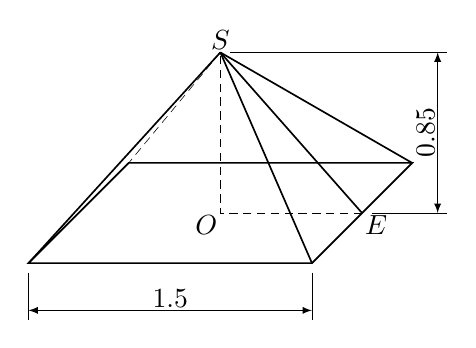
\begin{tikzpicture}[>=latex,scale=1.2,inner sep=1pt]
  \draw[very thin,densely dashed](1.5,0)node[below right]{$E$}--(0,0)node[below left]{$O$}--(0,1.7)node[above]{$S$};
  \draw[semithick](0,1.7)--(1.5,0);
  \draw[semithick](1.5,0)--++(45:0.75)coordinate(C)--++(-3,0)coordinate(D)--++(45:-1.5)coordinate(A)--++(3,0)coordinate(B)--cycle;
  \draw[semithick](0,1.7)--(A)(0,1.7)--(B)(0,1.7)--(C);
  \draw[very thin,densely dashed](0,1.7)--(D);
  \draw[very thin]([yshift=-1mm]A)--++(0,-0.5)([yshift=-1mm]B)--++(0,-0.5)(0.1,1.7)--(2.4,1.7)(1.6,0)--(2.4,0);
  \draw[very thin,<->]([yshift=-5mm]A)--([yshift=-5mm]B)node[midway,above]{1.5};
  \draw[very thin,<->](2.3,0)--(2.3,1.7)node[midway,above,sloped]{0.85};
\end{tikzpicture}
\end{document}